\documentclass[11pt, leqno, a4paper]{article}
\usepackage{hyperref, amsmath, amssymb, graphicx}
\hypersetup{colorlinks=true, urlcolor=blue, breaklinks=true}
\newcommand{\angles}[1]{$\langle$#1$\rangle$}

%%%%% ADD THIS TO YOUR PREAMBLE BEFORE LOADING Alegreya
\DeclareFontFamily{T1}{Alegreya-LF}{}
\newcommand{\adjustalegreya}{\fontdimen5\font=\fontcharht\font`x }
\makeatletter
\let\Alegreya@@scale\@empty
%%% uncomment the next line if you want to scale the font,
%%% changing the value to what suits you
% \def\Alegreya@@scale{s*[0.9]}%
\makeatother

\DeclareFontShape{T1}{Alegreya-LF}{k}{n}{
      <-> \Alegreya@@scale Alegreya-Black-lf-t1
}{\adjustalegreya}

\DeclareFontShape{T1}{Alegreya-LF}{k}{it}{
      <-> \Alegreya@@scale Alegreya-BlackItalic-lf-t1
}{\adjustalegreya}

\DeclareFontShape{T1}{Alegreya-LF}{k}{sl}{
      <-> ssub * Alegreya-LF/k/it
}{\adjustalegreya}

\DeclareFontShape{T1}{Alegreya-LF}{b}{n}{
      <-> \Alegreya@@scale Alegreya-Bold-lf-t1
}{\adjustalegreya}

\DeclareFontShape{T1}{Alegreya-LF}{b}{it}{
      <-> \Alegreya@@scale Alegreya-BoldItalic-lf-t1
}{\adjustalegreya}

\DeclareFontShape{T1}{Alegreya-LF}{b}{sl}{
      <-> ssub * Alegreya-LF/b/it
}{\adjustalegreya}

\DeclareFontShape{T1}{Alegreya-LF}{m}{n}{on the spot
      <-> \Alegreya@@scale Alegreya-Regular-lf-t1
}{\adjustalegreya}

\DeclareFontShape{T1}{Alegreya-LF}{m}{it}{
      <-> \Alegreya@@scale Alegreya-Italic-lf-t1
}{\adjustalegreya}

\DeclareFontShape{T1}{Alegreya-LF}{m}{sl}{
      <-> ssub * Alegreya-LF/m/it
}{\adjustalegreya}

\DeclareFontShape{T1}{Alegreya-LF}{bx}{sl}{
      <-> ssub * Alegreya-LF/b/sl
}{\adjustalegreya}

\DeclareFontShape{T1}{Alegreya-LF}{bx}{n}{
      <-> ssub * Alegreya-LF/b/n
}{\adjustalegreya}

\DeclareFontShape{T1}{Alegreya-LF}{bx}{it}{
      <-> ssub * Alegreya-LF/b/it
}{\adjustalegreya}

%%%% NOW YOU CAN SAFELY LOAD Alegreya (don't pass a scale option)
\usepackage{Alegreya}
\usepackage{amsmath}


\title{Final Project -- Basic Probability: Programming\\[2mm]
\large{2018-2019, Master of Logic, University of Amsterdam}}
\author{Instructors: Jakub Dotla\v{c}il}
\date{Submission deadline: December 16, 8pm}

\begin{document}
\maketitle

\section{Project Description}

In this project you will perform your own data analysis. Your task is
to use a technique known as linear regression (see below) to predict the median price of houses
in suburbs of Boston in the 1980s. The relevant information about the data can be found
\href{http://www.cs.toronto.edu/\%7Edelve/data/boston/bostonDetail.html}{here}. The variable that you need
to predict is stored in the last column, called MEDV.

This project will teach you two things: first, it introduces you to a continuous distribution, namely
the Gaussian. Linear regression and other Gaussian models are very useful in practice and you will
see them a lot when working with data. Second, you will have to interpret your results. Rather than
just running the algorithm, you will have to make sense of the algorithm's output.
\section{Data}

The data is present in the package \texttt{scikit-learn}. Install the package. After that, run:\\
\# Import the datasets\\
from sklearn import datasets\\[1em]
\# Load dataset that we will use\\
boston = datasets.load\_boston()\\[1em]
\# Create features variable matrix\\
features = boston.data\\[1em]
\# Collect the target variable (MEDV)\\
target = boston.target\\[1em]

In the features matrix, each row is one case. That is, each row represents information about one house. Each case has 13 features. The interpretation of each feature can be accessed by boston.DESCR. The values to be predicted (the median price of each house) are stored per case in target. For each case, you should try to combine the features you choose as predictors of the corresponding value in the target.

\section{Linear Regression}
To familiarise yourself with linear regression and its implementation, watch the
videos of Sections 2.1--4.5 (this is quite a lot of movies, but most of them just review linear algebra and can be skipped) of \href{https://www.youtube.com/watch?v=kHwlB_j7Hkc&list=PLLssT5z_DsK-h9vYZkQkYNWcItqhlRJLN&index=5&t=2s}{Andrew Ng's machine
learning course}. You can also sign up for \href{https://www.coursera.org/learn/machine-learning/home}{it on coursera} to see them
in higher resolution. Here, we will only shortly highlight the math of linear regression.

From a probabilistic view point, we assume that our data are independently distributed. This is a weaker
assumption than we have made so far because we do not assume that the distributions of our data points
are identical! In fact, linear regression is all about working with a different distribution for each
data point. 

In linear regression we assume that each data point $ x_{i},\ (1 \leq i \leq n) $ follows a 
\href{https://en.wikipedia.org/wiki/Normal_distribution}{Gaussian or normal distribution}. The probability
density function of this distribution is
\begin{equation}
P(x|\mu, \sigma^{2}) = \frac{1}{\sqrt{2\pi}\sigma}\exp\left(\frac{1}{2}\left(\frac{x - \mu}{\sigma}\right)^{2}\right) \ .
\end{equation}
What is special about the normal distribution is that its mean and variance are equal to its parameters.
In particular, we have $ \mathbb{E}[X] = \mu $ and $ \text{var}(X) = \sigma^{2} $ for 
$ X \sim \mathcal{N}(\mu, \sigma^{2}) $.

Linear regression assumes that the variance parameter $ \sigma^{2} $ is shared by all distributions
but that each data point $ x_{i} $ was generated from a Gaussian with mean $ \mu_{i} $. This mean
is computed as $ \mu_{i} = w^{\top}\vec{x_{i}} $ where $ w $ is a weight vector and $ \vec{x_{i}} $ is
a vector of predictors\footnote{For the sake of explanation, we make a strict difference between
features and predictors. Features are attributes of a data point whereas predictors are values
supplied to the model.} of $ x_{i} $. The mean is thus a linear combination of the data point's predictors.
Each coefficient in $ w $ relates its predictor linearly to the output variable.

\section{Your Task}

Your task is to implement linear regression for the Boston housing data set. You first implement a baseline regression model. A baseline of this study is the most basic implementation of the linear regression method on this dataset (you have to justify your choice of 
baseline!). Thereafter, you try to improve your model and get better predictions.

You have to submit a code that (i) runs linear regression on the dataset, (ii) specifies the baseline model, (iii) specifies the best model, and prints $R^{2}$ (see below) for both baseline and best model, (iv) plots a graph showing a relation between one variable (of your choosing) on the x-axis, and the predicted value on the y-axis.

\section{Evaluating Linear Regression}

Since linear regression makes continuous predictions, it cannot simply be evaluated on a wrong/correct
basis. The error of linear regression is induced by the distances of the predictions to the true values.
These distances are known as residuals. The sum of their squares is the (squared) error\footnote{Squaring
is necessary here because the negative and positive residuals would cancel each other out otherwise.}. 

\begin{figure}
    \begin{center}
    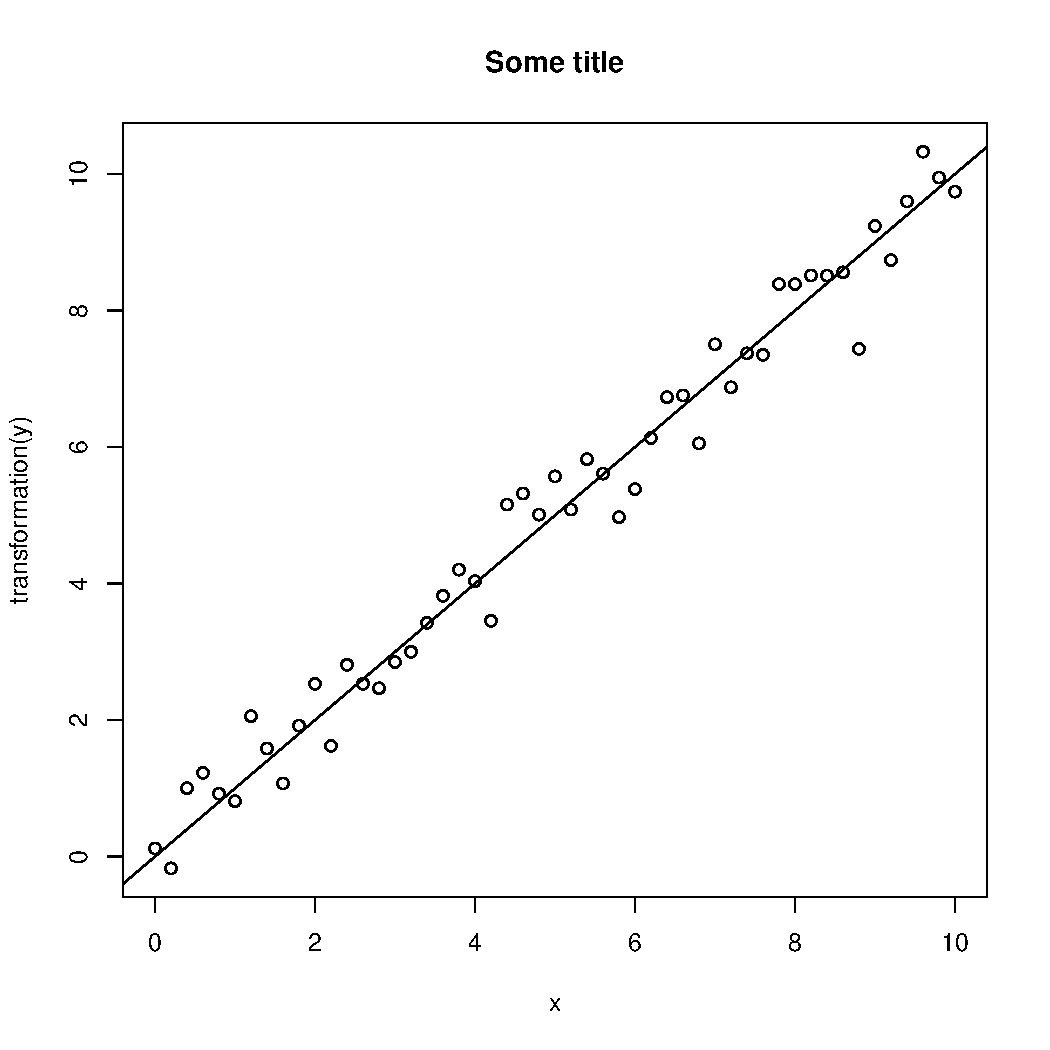
\includegraphics[width=0.5\textwidth]{plot.pdf}
    \end{center}
    \caption{Plot showing relationship between two variables\label{fig1}}
\end{figure}

Take a look at the plot in Fig.~\ref{fig1}. If the line was the output of a linear 
regression model, the residuals would be the vertical distances of the points to the line.

Since the residual error grows as a function of the number of data points, it is not a meaningful
way of evaluating a regression model. However, the residuals are again normally distributed. Standardly,
it is assumed that $ \mu=0 $ for that distribution.\footnote{This assumption is made because
residuals can be both positive and negative and there is no reason to assume that residuals should
be ``more positive'' or ``more negative'' on average.} If the
variance of their distribution is small, the regression line provides a tight approximation to the
true values. If the variance of that distribution is large, the approximation is pretty shabby. 

The standard quantity for assessing linear regression models is the 
\href{https://en.wikipedia.org/wiki/Coefficient_of_determination}{$ R^{2} $} which can be computed as
\begin{equation}
R^{2} = 1 - \frac{\sum_{i=1}^{n} \left( x_{i} - w^{\top}h(x_{i}) \right)^{2}}
{\sum_{i=1}^{n} \left(x_{i} - \frac{1}{n}\sum_{j = 1}^{n}x_{j}\right)^{2}} \ .
\end{equation}
Notice that the numerator is the sum of the residual errors 
and the denominator is the sample variance of the data.
The $ R^{2} $ thus expresses what fraction of the observed variance in the data is captured by the model. The 
$ R^{2} $ has the convenient property of being standardized, i.e.\ to
be bounded by 0 and 1. The better the linear regression fits the data,
the closer the value of $R^2$ is to 1.


\section{Types of Features and interpretation}

Roughly speaking there are two types of features: continuous ones and categorical ones.

\paragraph{Continuous Features} Let us assume that our model only has one continuous feature $ f $ 
with coefficient $ \alpha $. This means that for each point increase in $ f $, the predicted value
experiences a change of $ \alpha $. If $ \alpha $ was -2, the predicted value would decrease by two
for each point increase of $ f $. This is a general property of continuous features in linear
regression: their values are linearly related to the output value.

\paragraph{Categorical Features} Categorical features are all features for which the assumption
that their values are linearly related to the output does not make sense. Consider a feature \textit{gender}.
First of all, it needs to be turned into a number to be useful for regression. So let us
define the mapping $ \text{male} \mapsto 0, \ \text{female} \mapsto 1 $.\footnote{This mapping
is arbitrary in that we might also map males to 1 and females to 0.} Then we would certainly not
want to assume that the values of \textit{gender} are linearly related to whatever output we are dealing
with. Rather, it is the level\footnote{The values of categorical features are often called \textit{levels.}}
\textit{female} that causes a change in the output.

Whenever we are dealing with categorical features, we need to define a standard or default level. This
level can be chosen arbitrarily (in the example above it was chosen to be male). 
All coefficients of the other levels then have to be interpreted with
respect to that default. To make this concrete, let us assume that we model football-playing ability and
that our categorical features is \textit{nationality} with levels Holland, Germany and Switzerland.
We arbitrarily chose Holland as default. We then introduce two(!) predictors into the model, namely
Germany and Switzerland. Each of these predictors is either 1 (when the nationality matches the level)
or 0 (otherwise). After training our model, we get a coefficient of 5 for Germany and -3 for Switzerland.
The way to interpret these coefficients is that being German increases your ability in football by 5
compared to being Dutch whereas being Swiss decreases it by 3 (again compared to being Dutch).

The reason that we need to introduce 3 levels when dealing with 2 predictors is that if we assigned
the numbers 1 and 2 to Germany and Switzerland, we would again assume a linear relationship based on
nationality. In general, introducing a predictor for each non-standard level allows us to estimate a separate coefficient
per level.

A pre-final remark: it is not always clear whether a feature should be seen as continuous or categorical.
In the housing data, we have the RAD feature. Should that be continuous or categorical? This is
something you may want to experiment with.

\section{Learning}

Learning a linear regression model can be done with the technique of least squares. This basically
means that you try to iteratively minimise the sum of squares of the residuals. The details are
explained in the videos.

\section{Improving your Algorithm}

There are several ways to improve your algorithm. As discussed in the videos, you may use regularisation.
You can also try to build new predictors by transforming or combining features. All of this
is up to you. The important thing is that in the end you can show a real improvement through an
increase in $ R^{2} $.

\section{Deliverables}
\begin{itemize}
\item \textbf{Code:} A code that you have written, collected in one python file. This code should be executable either from the command line or from Pycharm (or both).
\item The code can use libraries (numpy, matplotlib), but \emph{it must not use a previously implemented linear regression}! You have to build the regression yourself.
\item Readme file: The file specifies how to run the code if necessary (for example, because running it requires optional arguments). The file should also shortly summarize what you picked as the baseline model, what you picked as the final model, and (very shortly) why you made this choice.
\end{itemize}

\section{Assessment}
The lecturer of the course determines the final grade for the project.

Here is the break-down of what I consider:
\begin{itemize}
    \item 2 points: The code should be well documented, so that I can understand what each class and method and function does. The code should run (from Pycharm or command line) and (at least) print the baseline model and its $R^2$, the best model and its $R^2$, and plot at least one graph.
    \item 3 points: Linear regression is implemented correctly and it works with numpy arrays (e.g., it does not loop through lists).
    \item 1 point: Plotting function works and it plots a graph showing the relation between (some subset of) features and the target variable. The data points are printed as dots and the linear regression fit is also shown in the graph.
    \item 1 point: The best model has $R^2$ higher than 0.7
    \item 1 point: The best model has $R^2$ higher than 0.75
    \item 1 point: The best model has $R^2$ higher than 0.8
    \item 1 point: Description and discussion in the readme file is followable, it is explained what the baseline and best models are. 
\end{itemize}


\end{document}
